\documentclass[12pt]{report}
\usepackage[utf8]{inputenc}
\usepackage[russian]{babel}
%\usepackage[14pt]{extsizes}
\usepackage{listings}
\usepackage{graphicx}
\usepackage{amsmath,amsfonts,amssymb,amsthm,mathtools} 
\usepackage{pgfplots}
\usepackage{filecontents}
\usepackage{indentfirst}
\usepackage{eucal}
\usepackage{enumitem}
\frenchspacing

\usepackage{indentfirst} % Красная строка


\usetikzlibrary{datavisualization}
\usetikzlibrary{datavisualization.formats.functions}

\usepackage{amsmath}




% Для листинга кода:
\lstset{ %
language=python,                 % выбор языка для подсветки
basicstyle=\small\sffamily, % размер и начертание шрифта для подсветки кода
numbers=left,               % где поставить нумерацию строк (слева\справа)
numberstyle=\tiny,           % размер шрифта для номеров строк
stepnumber=1,                   % размер шага между двумя номерами строк
numbersep=5pt,                % как далеко отстоят номера строк от подсвечиваемого кода
showspaces=false,            % показывать или нет пробелы специальными отступами
showstringspaces=false,      % показывать или нет пробелы в строках
showtabs=false,             % показывать или нет табуляцию в строках
frame=single,              % рисовать рамку вокруг кода
tabsize=2,                 % размер табуляции по умолчанию равен 2 пробелам
captionpos=t,              % позиция заголовка вверху [t] или внизу [b] 
breaklines=true,           % автоматически переносить строки (да\нет)
breakatwhitespace=false, % переносить строки только если есть пробел
escapeinside={\#*}{*)}   % если нужно добавить комментарии в коде
}

\usepackage[left=2cm,right=2cm, top=2cm,bottom=2cm,bindingoffset=0cm]{geometry}
% Для измененных титулов глав:
\usepackage{titlesec, blindtext, color} % подключаем нужные пакеты
\definecolor{gray75}{gray}{0.75} % определяем цвет
\newcommand{\hsp}{\hspace{20pt}} % длина линии в 20pt
% titleformat определяет стиль
\titleformat{\chapter}[hang]{\Huge\bfseries}{\thechapter\hsp\textcolor{gray75}{|}\hsp}{0pt}{\Huge\bfseries}


% plot
\usepackage{pgfplots}
\usepackage{filecontents}
\usetikzlibrary{datavisualization}
\usetikzlibrary{datavisualization.formats.functions}

\begin{document}
\thispagestyle{empty}
\begin{titlepage}
	\noindent \begin{minipage}{0.15\textwidth}
	
\includegraphics[width=\linewidth]{b_logo}
	\end{minipage}
	\noindent\begin{minipage}{0.9\textwidth}\centering
		\textbf{Министерство науки и высшего образования Российской Федерации}\\
		\textbf{Федеральное государственное бюджетное образовательное учреждение высшего образования}\\
		\textbf{~~~«Московский государственный технический университет имени Н.Э.~Баумана}\\
		\textbf{(национальный исследовательский университет)»}\\
		\textbf{(МГТУ им. Н.Э.~Баумана)}
	\end{minipage}
	
	\noindent\rule{18cm}{3pt}
	\newline\newline
	\noindent ФАКУЛЬТЕТ $\underline{\text{«Информатика и системы управления»}}$ \newline\newline
	\noindent КАФЕДРА $\underline{\text{«Программное обеспечение ЭВМ и информационные технологии»}}$\newline\newline\newline\newline\newline
	
	
	\begin{center}
		\noindent\begin{minipage}{1.3\textwidth}\centering
			\Large\textbf{  Отчет по лабораторной работе №6}\newline
			\textbf{по дисциплине "Анализ алгоритмов"}\newline\newline
		\end{minipage}
	\end{center}
	
	\noindent\textbf{Тема} $\underline{\text{Муравьиный алгоритм}}$\newline\newline
	\noindent\textbf{Студент} $\underline{\text{Андрич К. }}$\newline\newline
	\noindent\textbf{Группа} $\underline{\text{ИУ7И-56Б}}$\newline\newline
	\noindent\textbf{Оценка (баллы)} $\underline{\text{~~~~~~~~~~~~~~~~~~~~~~~~~~~}}$\newline\newline
	\noindent\textbf{Преподаватели} $\underline{\text{Волкова Л.Л.}}$\newline\newline\newline
	
	\begin{center}
		\vfill
		Москва~---~\the\year
		~г.
	\end{center}
\end{titlepage}


\tableofcontents

\newpage
\chapter*{Введение}
\addcontentsline{toc}{chapter}{Введение}
Задача коммивояжера применяется в различных сферах, таких как: маршрутизация транспортных
потоков и выбор оптимальной траектории движения рабочего инструмента, а
также в сферах, которые на первый взгляд не связаны с маршрутизацией:
секвенирования нуклеотидных последовательностей биополимеров,
эвристического определения схожести строк, построения практических
алгоритмов исследования специально определённых бесконечных
грамматических структур и построения эволюционных деревьев.
\newline

Муравьиный алгоритм (алгоритм оптимизации подражанием муравьиной колонии) — один из полиномиальных алгоритмов для нахождения приближённых решений задачи коммивояжёра, а также решения аналогичных задач поиска маршрутов на графах. Алгоритм называется полиномиальным (имеющим полиномиальную временную сложность), если существует полином $p(x)$ такой, что на любом входном слове длины $n$ алгоритм завершает вычисления после выполнения не более чем $p(n)$ операций .
\newline

Целью работы работы является проведение сравнительного анализа метода полного перебора и эвристического метода на базе муравьиного алгоритма.
\newline

Для достижения цели ставятся следующие задачи:
\begin{itemize}
	\item изучить метод полного перебора и метод на базе муравьиного алгоритма для решения задачи коммивояжёра;
	\item реализовать метод полного перебора и метод на базе муравьиного алгоритма для решения задачи коммивояжёра;
	\item провести параметризацию метода на базе муравьиного алгоритма для выбранного класса задач, т.е. определить такие комбинации параметров или их диапазонов, при которых метод даёт наилучшие результаты на выбранном классе задач;
	\item сравнить алгоритм полного перебора и муравьиный по скорости работы.
\end{itemize}

\chapter{Аналитическая часть}

В данной части будут рассмотрены основные теоретические аспекты, связанные с задачей коммивояжера.

\section{Задача коммивояжера}

Задача коммивояжера формулируется просто: на плоскости (в пространстве) расположены N городов, заданы расстояния между каждой парой городов. Требуется найти маршрут минимальной длины с посещением каждого города ровно один раз и с возвращением в исходную точку. Необходимо дополнительно учитывать расстояния от города до города, которые предполагаются известными. Эти «расстояния» можно заменить на количество затраченного времени, стоимость проезда или предполагать другие произвольные значения. 
\newline

На графах задача формулируется следующим образом: требуется найти гамильтонов цикл наименьшей стоимости во взвешенном полном графе. Т.е. выйдя из стартовой вершины, посетить каждую вершину графа ровно один раз и вернуться в начальную по кратчайшему пути.
\newline

Гамильтонов путь – путь, содержащий каждую вершину графа ровно один раз. Гамильтонов путь, начальная и конечная вершины которого совпадают, называется гамильтоновым циклом.

\section{Муравьиный алгоритм}

Муравьинный алгоритм – один из алгоритмов нахождения решений задачи коммивояжера. 

Алгоритм основывается на поведении муравьев в поиске кратчайшего пути от колонии до источника питания. Моделирование поведения муравья связано с распределением феромонов на пути (на ребре в данном случае), количество феромона пропорционально длине маршрута. Таким образом, чем короче найденный маршрут, тем больше будет на нем феромонов. Чтобы алгоритм не сводился к единственному варианту, вводится «испарение» феромонов с пути со временем.


Муравьинный алгоритм использует три основных понятия:

\begin{enumerate}
	
	\item память муравья – список вершин, которые он уже посетил; также есть список $J_{i,k}$ – список вершин, которые нужно посетить $i$-тому муравью, находящемуся в вершине $k$;
	
	\item видимость – обратная расстоянию величина, $\eta = \frac{1}{D_{i,j}}$ , где $D_{i,j}$ – расстояние между вершинами $i$ и $j$;
	
	\item феромонный след – «опыт» муравьев, коэффициент вероятности того, что муравей захочет перейти из вершины $i$ в $j$ – $\tau_{i,j}$.
	
\end{enumerate}


Вероятность перехода муравья $k$ в вершину $j$ из вершины $i$ рассчитывается по формуле \ref{eq1}:

\begin{equation}
	\label{eq1} 
	\begin{matrix}
		P_{i,j,k}(t) & = 
		& \left\{
		\begin{matrix}
			\frac{[\tau_{i,j}(t)]^\alpha * [\eta_{i,j}]^\beta}{\sum\limits_{l = J_{i,k}} [\tau_{i,j}(t)]^\alpha * [\eta_{i,j}]^\beta }   & j \in J_{i,k} \\
			0 & j \notin J_{i,k} \\
		\end{matrix} \right. 
	\end{matrix}
\end{equation}

$\alpha, \beta$ – весовые коэффициенты, которые задают важность феромона и привлекательность ребра.

Если $\alpha = 0$, то алгоритм становится «жадным», если $\beta = 0$, то муравьи оказываются «слепы» и опираются только на феромонный след.


Пройдя ребро $(i, j)$, муравей откладывает на нем некоторое количество феромона, которое рассчитывается по формуле \ref{eq2}:

\begin{equation}
	\label{eq2} 
	\begin{matrix}
		\Delta\tau_{i,j,k}(t) & = 
		& \left \{
		\begin{matrix}
			\frac{Q}{L_k(t)}, & (i,j) \in T_k(t) \\
			0, & (i,j) \notin T_k(t) \\
		\end{matrix} \right.
	\end{matrix}
\end{equation}\\

$p$ - коэффициент испарения феромона; 

$Q$ - значение порядка длины оптимального пути; 

$L_k$ - длина маршруту, пройденная муравьем $k$ к моменту времени $t$;\\

Пусть $p \in [0, 1]$ - коэффициент испарения, тогда правило испарения имеет вид (формула \ref{eq3}):  

\begin{equation}
	\label{eq3} 
	\tau_{i,j}(t+1) = (1-p)*\tau_{i,j}(t) + \Delta\tau_{i,j}(t); \Delta\tau_{i,j}(t) = \sum\limits_{k = 1}^{m} \Delta\tau_{i,j,k}(t)
\end{equation} 

где $m$ - количество муравьев в колонии.

\section{Вывод}
	В данном разделе поставлена цель и описаны задачи и теоретическая часть муравьиного алгоритма и полного перебора.
	
	
\clearpage

\chapter{Конструкторская часть}

\section{Схемы алгоритмов}

На рисунках \ref{img:main} - 2.3 представлены схемы алгоритмов полного перебора и муравьиного алгоритма.

	\begin{center}
	\label{img:main} 
	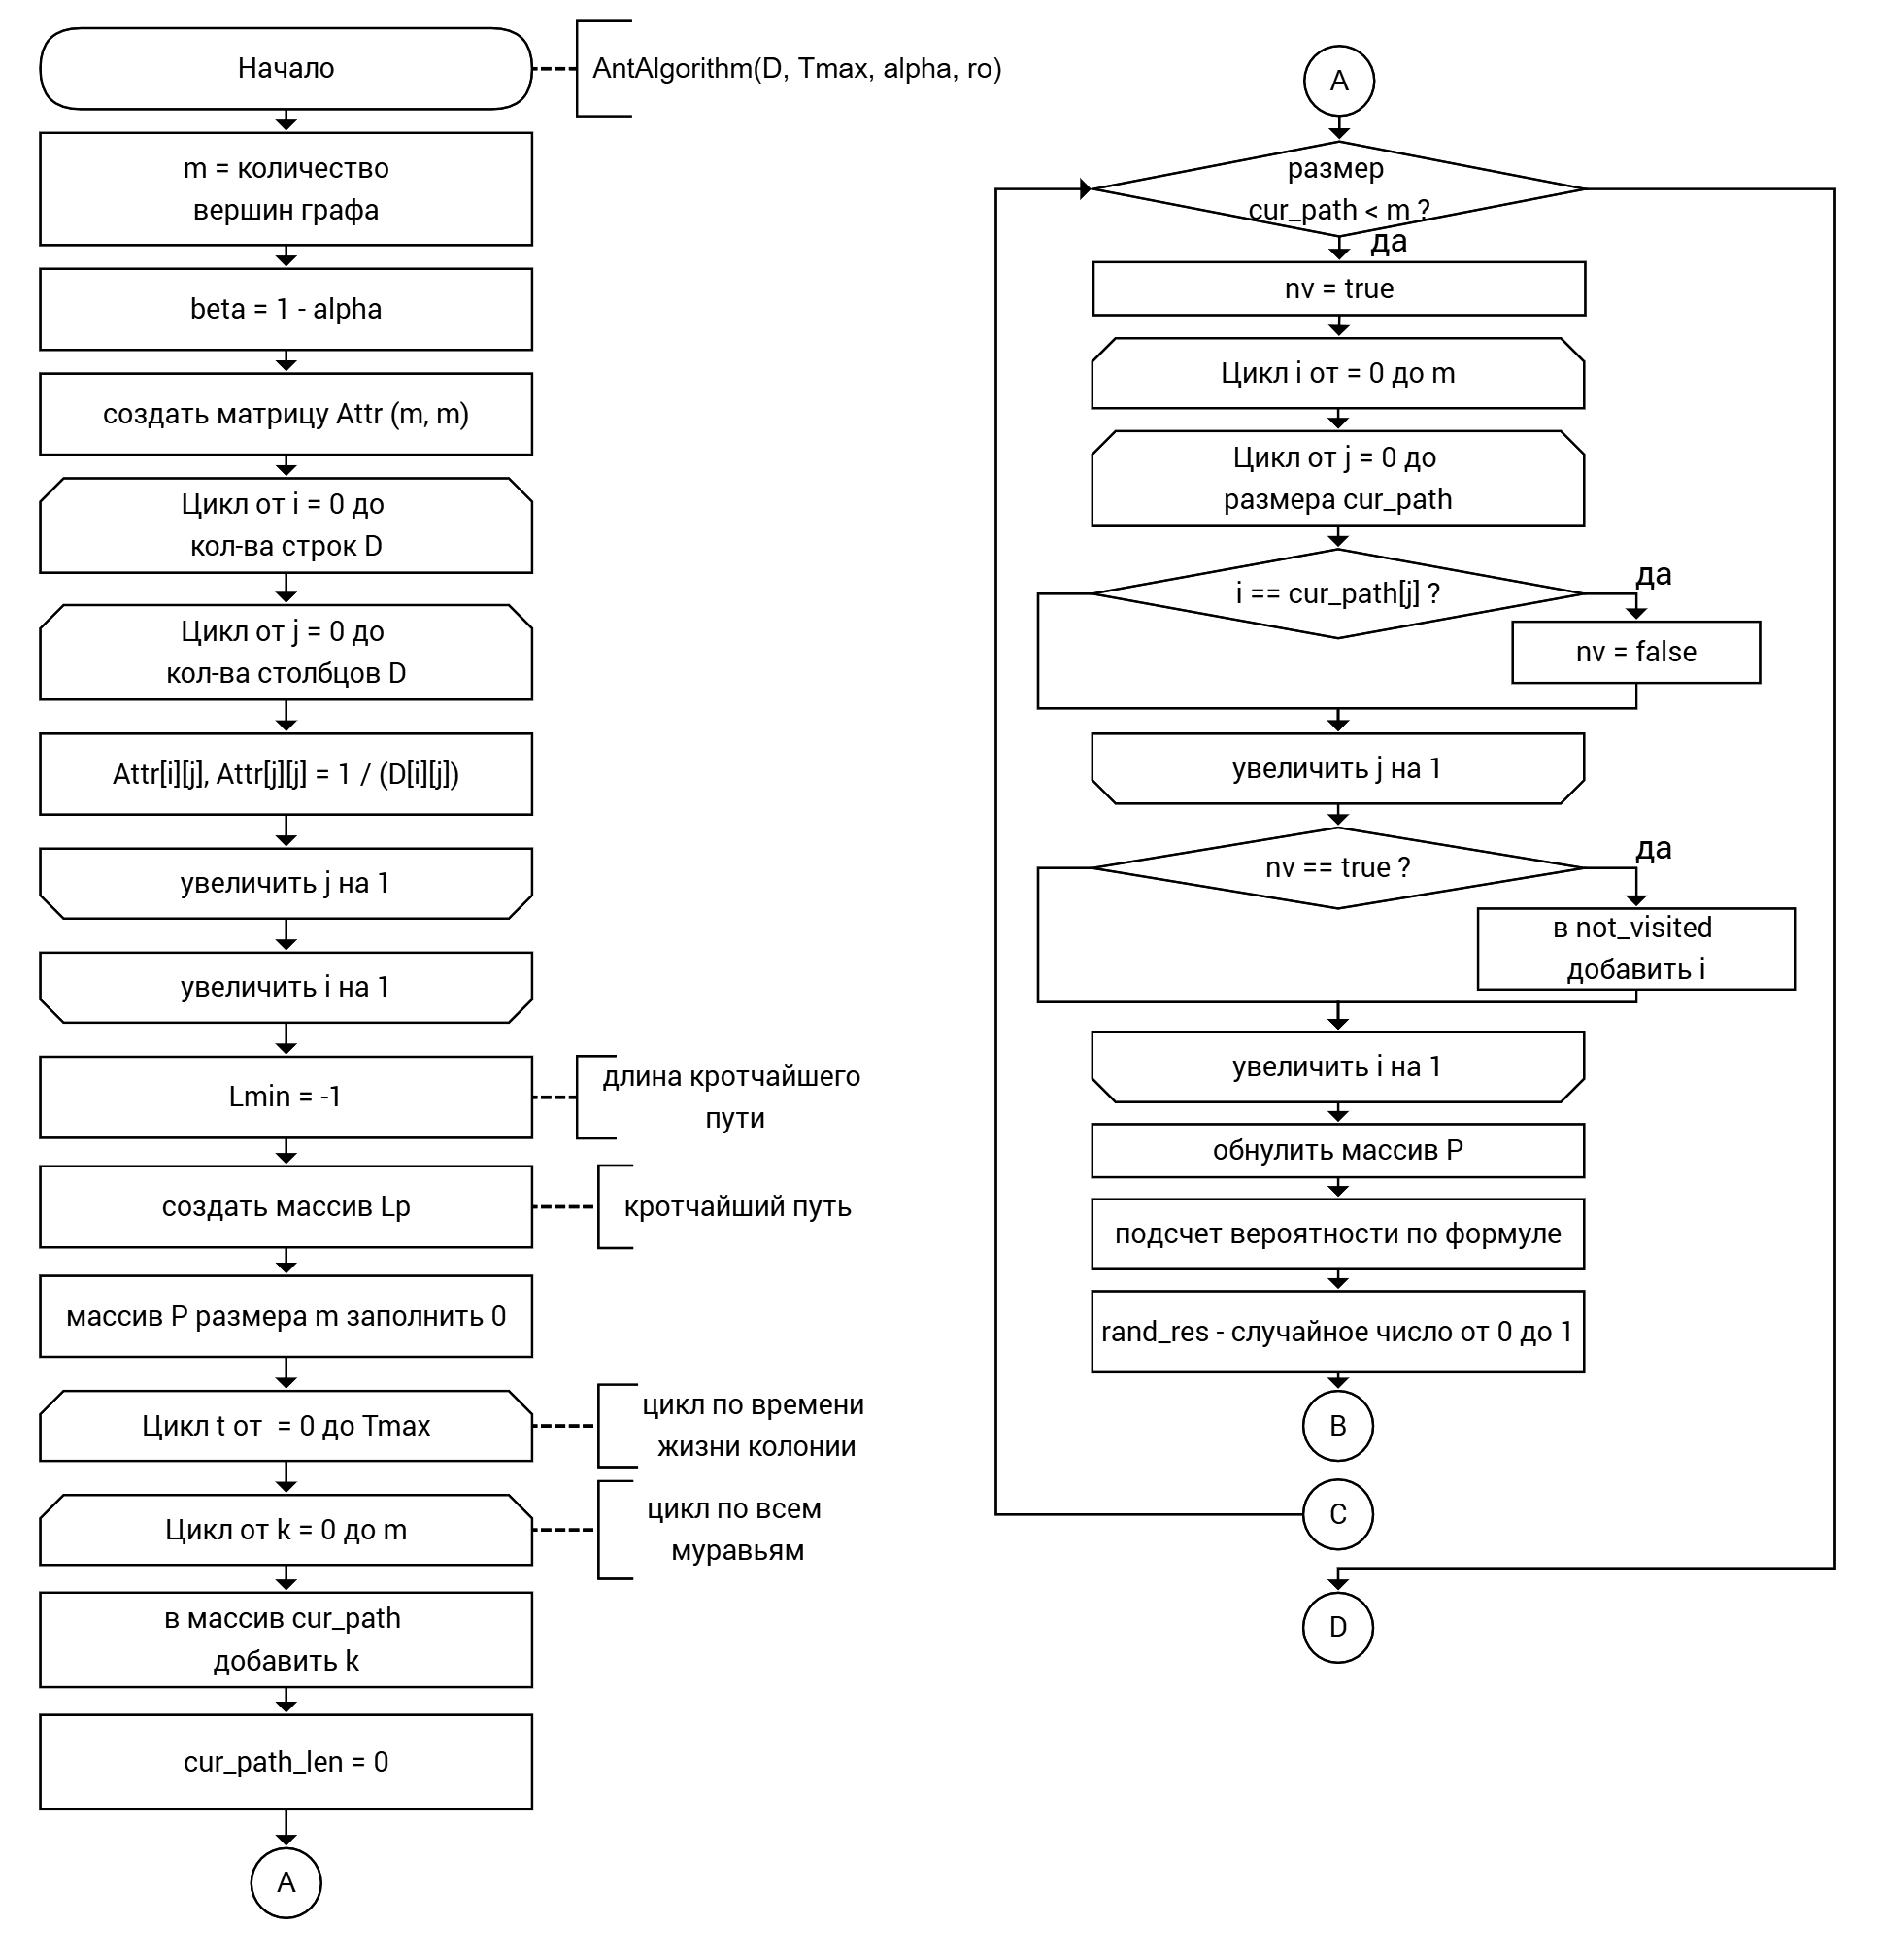
\includegraphics[scale = 0.3]{ant_1} \\ Рисунок 2.1 - Муравьиный алгоритм (часть 1)
\end{center}

\begin{center}
	\label{img:subr} 
	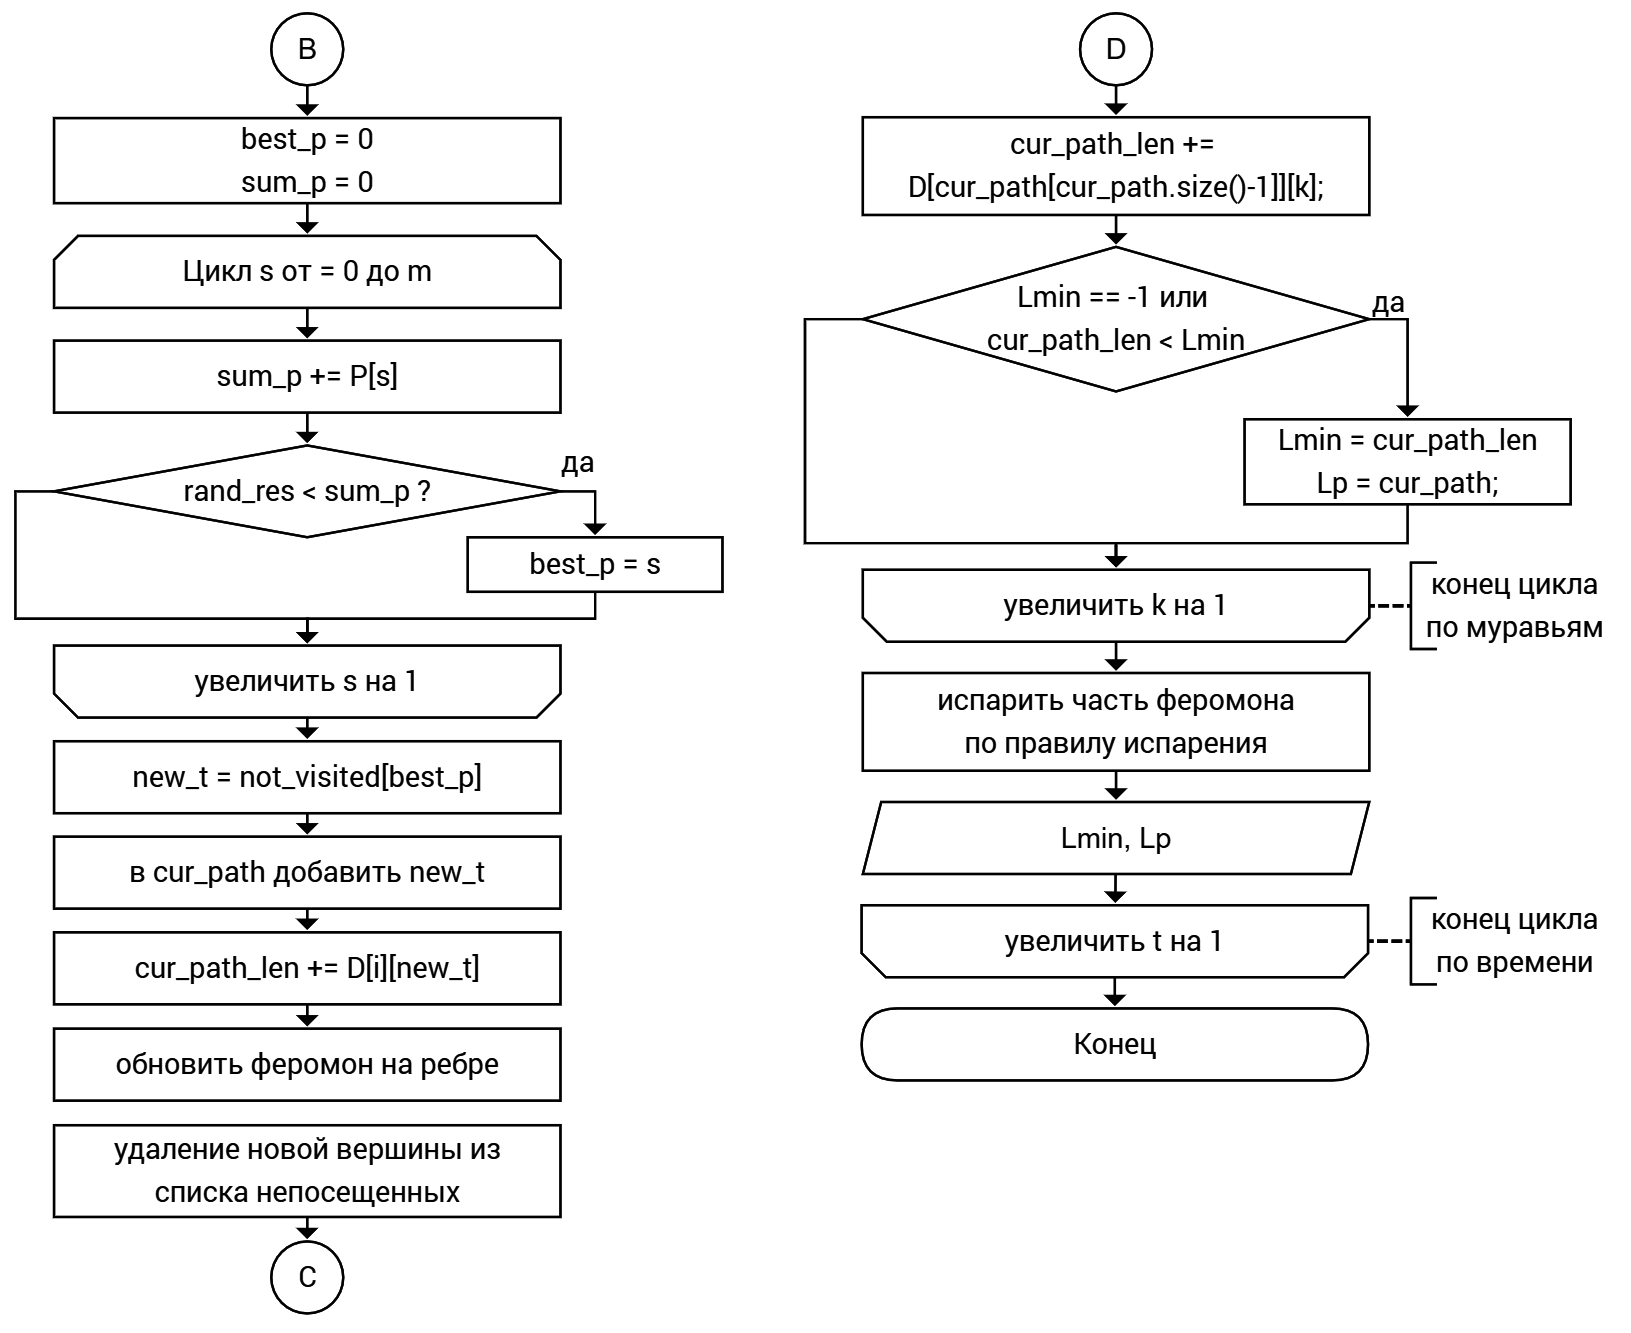
\includegraphics[scale = 0.42]{ant_2} \\ Рисунок 2.2 - Муравьиный алгоритм (часть 2)
\end{center}

\begin{center}
	\label{img:vin_opt} 
	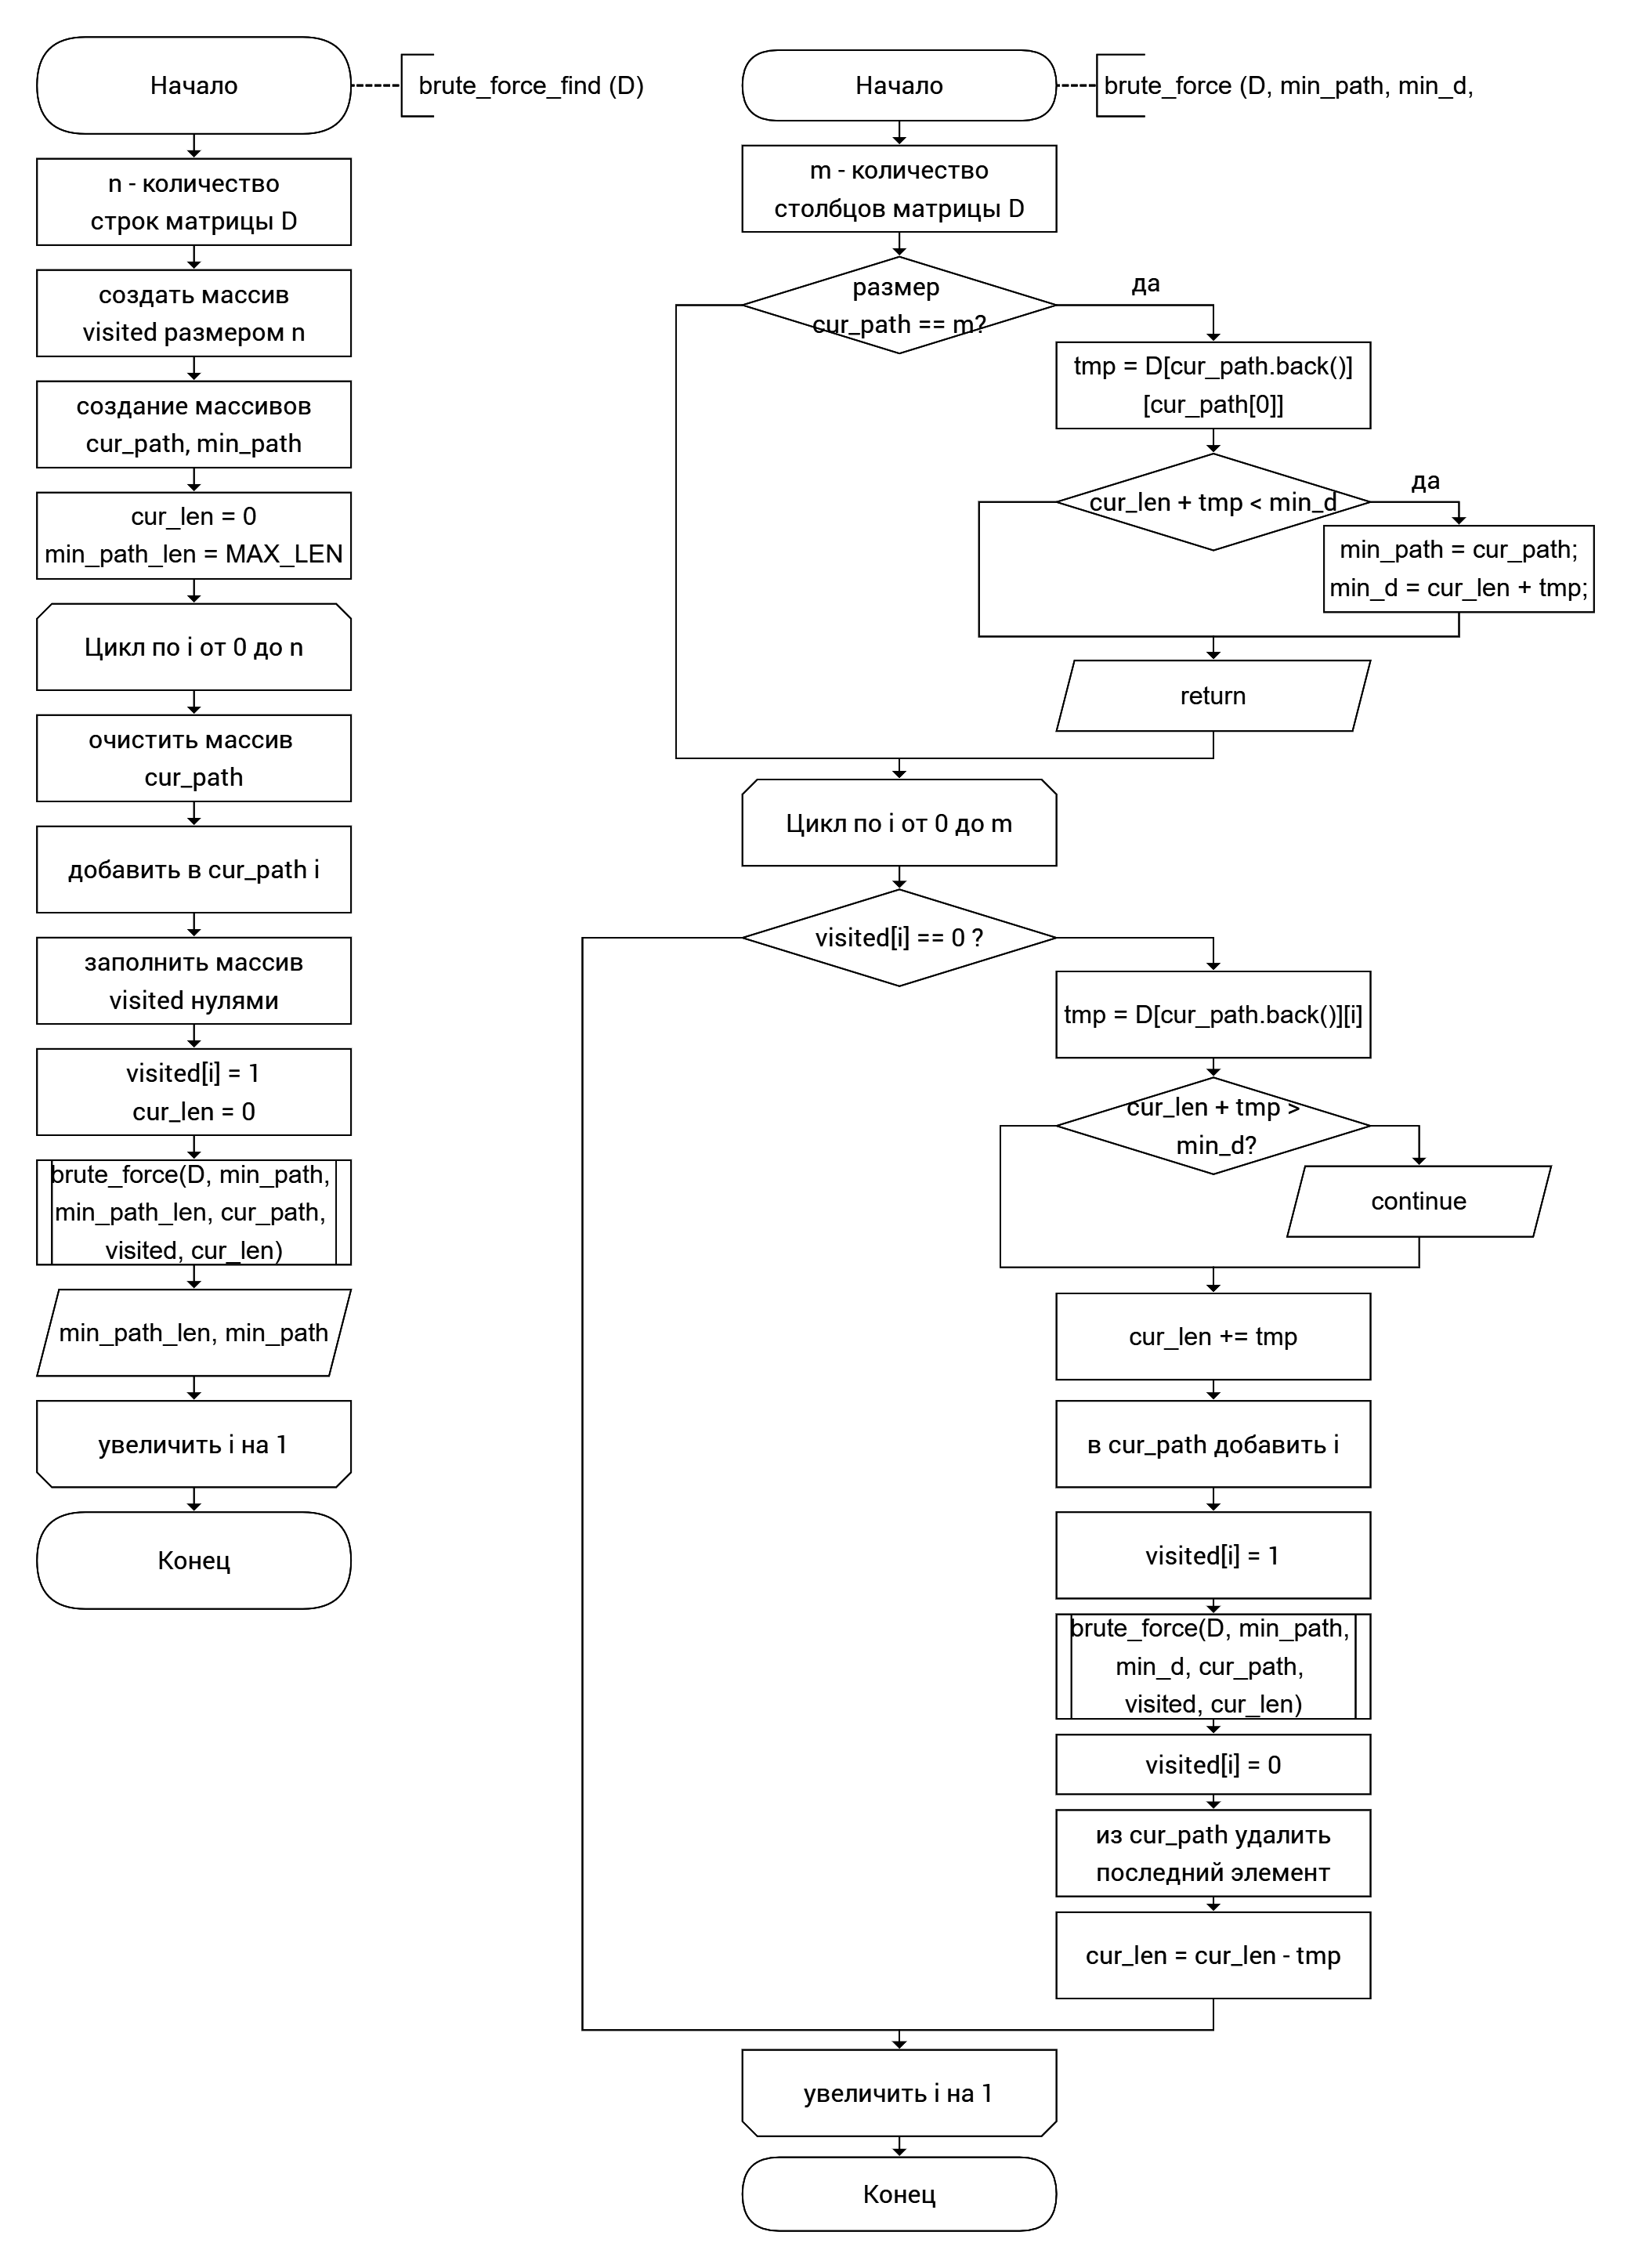
\includegraphics[scale = 0.3]{brute} \\ Рисунок 2.3 - Алгоритм полного перебора
\end{center}


\section{Требования к программному обеспечению}

На входе программа принимает матрицу смежности графа. На выходе ПО должно обеспечить вывод замеров времени работы алгоритма полного перебора и муравьиного алгоритма, выводить на экран длину самого короткого пути (стоимость обхода) и сам путь.

\section{Оценка трудоемкости муравьиного алгоритма}

Ниже приведены теоретические оценки трудоемкости муравьиного алгоритма.

\begin{enumerate}
	\item[1)] Трудоемкость цикла поиска непосещенных вершин (формула \ref{eq:eq1}):
	\begin{equation}
		\label{eq:eq1}
		f_1 = 1 + 2 + N \cdot (2 + 1 + 2 + 1 + S \cdot (3 + 1 + 1 + 1) + 1 + 1) = 3 + 6 \cdot N \cdot S + 8 \cdot N
	\end{equation}
	
	\item[2)]
	Трудоемкость цикла подсчета вероятности (формула \ref{eq:eq2}):
	$$f_2 = 2 + N \cdot (2 + 1 + 1) + 2 + S \cdot (2 + 3 + 1 + 1 + 2 + S \cdot (2 + 4 + 2 + 1) + 1 + 7 + 2 + 1 + 1) $$
	\begin{equation}
		\label{eq:eq2}
		f_2 = 4 + 3 \cdot N + 21 \cdot S + 9 \cdot S^{2}
	\end{equation}
	
	\item[3)]
	Трудоемкость цикла вычисления нового города, в которую попадет муравей (формула \ref{eq:eq3}):
	\begin{equation}
		\label{eq:eq3}
		f_3 = 4 + 2 + 2 + N \cdot (2 + 2 + 3 + 2) = 8 + 9 \cdot N
	\end{equation}
	
	\item[4)]
	Трудоемкость цикла, в которром происходит испарение феромона (формула \ref{eq:eq4}):
	\begin{equation}
		\label{eq:eq4}
		f_4 = 2 + N \cdot (2 + 2 + N \cdot (2 + 6 + 4 + 2 + 1 + 3)) = 2 + 4 \cdot N + 18 \cdot N^{2}
	\end{equation}
	
	\item[5)]
	Трудоемкость оснвоного цикла по времени жизни колонии (формула \ref{eq:eq5}):
	
	\begin{center}
		$f_5 = 2 + T_{max} \cdot (3 + 2 + M \cdot (2 + 1 + 1 + 2 + 1 +$
		$N \cdot [1 + 1 + f_1 + f_2 + f_3 + 2 + 1 + 3 + 4 + 1] + 3 
		+ 6 + 3 + 2) + f_4)$
	\end{center}
	
	\begin{center}
		$f_5 = 2 + T_{max} \cdot (5 + M \cdot (7 + N \cdot [2 + 3 + 6 \cdot N \cdot S +$
		$ + 8 \cdot N + 4 + 3 \cdot N + 21 \cdot S + 9 \cdot S^{2} + 8 + 9 \cdot N + 11] + 14) + 2 + 4 \cdot N + 18 \cdot N^{2})$
	\end{center}
	
	\begin{equation}
		\label{eq:eq5}
		f_5 = 2 + T_{max} \cdot (7 + M \cdot (21 + N \cdot (28 + 21 \cdot S + 9 \cdot S^{2}) + N^{2} \cdot (20 + 6 \cdot S)) + 4 \cdot N + 18 \cdot N^{2})
	\end{equation}
	
\end{enumerate}

Таким образом, сложность муравьиного алгоритма равна $O(T_{max} \cdot M \cdot N^{2})$. 

С учетом того, что в моей реализации алгоритма в каждом городе находится 1 муравей, сложность алгоритма равна $O(T_{max} \cdot N^{3})$.

\section{Вывод}
	На основе теоретических данных, полученные в аналитическом разделе были построены схемы иследуеммых  алгоритмов и показана оценка трудоемкости муравьиного алгоритма.

\chapter{Технологическая часть}

\section{Выбор ЯП}
 В качестве языка программирования был выбран $C++$ \cite{link4}, так как я имею опыт написания программ на данном языке. В качестве среды разработки выбран $Visual Studio$.

\section{Реализация алгоритмов}

В листингах 3.1 - 3.4 представлена реализация алгоритма полного перебора и муравьиного алгоритма.

\begin{lstlisting}[label=some-code,caption=Реализация алгоритма полного перебора (нерекурсивная часть),language=C++]
pair<int, vector<int> > brute_force_find(Matrix D)
{
	int n = D.rows();
	vector<bool> visited(n, 0);
	vector<int> cur_path;
	vector<int> min_path;
	int cur_len = 0;
	int min_path_len = MAX_LEN;
	for (int i = 0; i < n; i++)
	{
		cur_path.clear();
		cur_path.push_back(i);
		fill(visited.begin(), visited.end(), 0);
		visited[i] = 1;
		cur_len = 0;
		brute_force(D, min_path, min_path_len, cur_path, visited, cur_len);
	}
	return pair<int, vector<int>>(min_path_len, min_path);
}
\end{lstlisting}

\newpage

\begin{lstlisting}[label=some-code,caption=Реализация алгоритма полного перебора (рекурсивная часть),language=C++]
void brute_force(Matrix &D, vector<int> &min_path, int &min_d, vector<int> &cur_path, vector<bool> &visited, int &cur_len) {
	size_t M = D.cols();
	if (cur_path.size() == M) {
		ss++;
		int tmp = D[cur_path.back()][cur_path[0]];
		if (cur_len + tmp < min_d)
		{
			min_path = cur_path;
			min_d = cur_len + tmp;
		}
		return;
	}
	for (size_t i = 0; i < M; i++) {
		if (!visited[i])
		{
			int tmp = D[cur_path.back()][i];
			if (cur_len + tmp > min_d)
			continue;
			cur_len += tmp;
			cur_path.push_back(i);
			visited[i] = 1;
			brute_force(D, min_path, min_d, cur_path, visited, cur_len);
			visited[i] = 0;
			cur_path.pop_back();
			cur_len -= tmp;
		}
	}
}
\end{lstlisting}

\newpage

\begin{lstlisting}[label=some-code,caption=Реализация муравьиного алгоритма част 1,language=C++]
pair<int, vector<int>> AntAlgorithm(Matrix D, const int Tmax, const double alpha, const double ro){
	const int teta_beg = 10;
	const int teta_min = 5;
	const size_t M = D.cols(); 
	const double Q = D.avg() * M; 
	const double betta = 1 - alpha;
	
	Matrix Attr(M, M); 
	for (size_t i = 0; i < D.rows(); i++){
		for (size_t j = 0; j < D.cols(); j++) {
			double tmp = 1/D[i][j];
			Attr[i][j] = tmp;
			Attr[j][i] = tmp;
		}
	}
	Matrix Teta(M, M, teta_beg); 
	Matrix Delta_Teta(M, M); 
	
	int Lmin = -1; 
	vector<int> Lp; 
	vector<double> P(M, 0.0); 
	
	double random_res;
	for (int t = 0; t < Tmax; t++) {
		Delta_Teta.zero();
		for (size_t k = 0; k < M; k++) {
			vector<int> cur_path;
			cur_path.push_back(k);
			int cur_path_length = 0;
			int i = k;
			while (cur_path.size() < M) {
				vector<int> not_visited;
				bool nv = true;
				for (size_t i = 0; i < M; i++) {
					nv = true;
					for (size_t j = 0; j < cur_path.size(); j++) {
						if ((int)i == cur_path[j]) nv = false;
					}
					if (nv)
					not_visited.push_back(i);
				}
				for (size_t j = 0; j < M ; j++){
					P[j] = 0.0;
				}
\end{lstlisting}

\newpage

\begin{lstlisting}
				for (size_t j = 0; j < not_visited.size(); j++) {
					if (D[i][not_visited[j]]) {
						double sum = 0;
						for (auto n: not_visited) {
							sum += pow(Teta[i][n], alpha) * pow(Attr[i][n], betta);
						}
						P[j] = pow(Teta[i][not_visited[j]], alpha) * 		pow(Attr[i][not_visited[j]], betta)/sum;
					}
					else {
						P[j] = 0;
					}
				}
				random_res  = (rand() % 100) / 100.0;
				int best_p = 0;
				double sum_p = 0;
				for (size_t s = 0; s < M; s++) {
					sum_p += P[s];
					if(random_res < sum_p)
					{
						best_p = s;
						break;
					}
				}
				int new_town = not_visited[best_p];
				cur_path.push_back(new_town);
				cur_path_length += D[i][new_town];
				
				Delta_Teta[i][new_town] += Q/cur_path_length;
				
				i = new_town; 
				not_visited.erase(not_visited.begin()+best_p);
			}
			cur_path_length += D[cur_path[cur_path.size()-1]][k];
			if (Lmin == -1 || cur_path_length < Lmin){
				Lmin = cur_path_length;
				Lp = cur_path;
			}
		}
		for (size_t k = 0; k < M; k++) {
			for (size_t h = 0; h < M; h++) {
				Teta[k][h] = Teta[k][h] * (1.0 - ro) + Delta_Teta[k][h];
				if (Teta[k][h] < teta_min){
						Teta[k][h] = teta_min;
				}
			}
		}
	}
return pair<int, vector<int>>(Lmin, Lp); }
\end{lstlisting}

\section{Тестовые данные}

	В таблице 3.1 представлена заготовка данных для тестирования по методу черного ящика алгоритма полного перебора и муравьиного алгоритма.

	\begin{center}
	Таблица 3.1 -- Подготовленные тестовые данные
\end{center}

\begin{center}
	\begin{table}[h!]
		\begin{center}
			\begin{tabular}{|l|l|l|}
				\hline
				\multicolumn{1}{|c|}{Матрица}                                                                     & \begin{tabular}[c]{@{}l@{}}Алгоритм\\ полного перебора\end{tabular}                               & \begin{tabular}[c]{@{}l@{}}Муравьиный\\ алгоритм\end{tabular}                                     \\ \hline
				\begin{tabular}[c]{@{}l@{}}0 9 8 2 9\\ 9 0 1 7 4\\ 8 1 0 7 3\\ 2 7 7 0 8\\ 9 4 3 8 0\end{tabular} & \begin{tabular}[c]{@{}l@{}}Минимальная длина пути = 22\\ Минимальный путь: 0 3 1 2 4\end{tabular} & \begin{tabular}[c]{@{}l@{}}Минимальная длина пути = 22\\ Минимальный путь: 0 3 1 2 4\end{tabular} \\ \hline
				\begin{tabular}[c]{@{}l@{}}0 7 7\\ 7 0 3\\ 7 3 0\end{tabular}                                     & \begin{tabular}[c]{@{}l@{}}Min path length = 17\\ Минимальный путь: 0 1 2\end{tabular}            & \begin{tabular}[c]{@{}l@{}}Min path length = 17\\ Минимальный путь: 0 1 2\end{tabular}            \\ \hline
			\end{tabular}
		\end{center}
	\end{table}
\end{center}

\section{Вывод}
Реализованы алгоритм полного перебора и муравьиный алгоритм, подготовлены тесты для оценки качества их работы.

В результате тестирования рассматриваемые алгоритмы вывели на экран ожидаемые результаты тестов. 

\chapter{Исследовательская часть}

 В данной части производится экспериментальное сравнение времени работы алгоритма полного перебора и муравьиного алгоритма. Также рассматривается параметризация муравьиного алгоритма.

\section{Пример работы}

	На рисунках 4.1 и 4.2 представлены примеры работы программы на матрицах разного размера: выводится матрица смежности, длина самого короткого пути и сам путь для алгоритма полного перебора и для муравьиного алгоритма.
\begin{center}
	\label{img:prim} 
	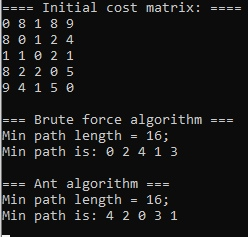
\includegraphics[scale = 1]{primer1} \\ Рисунок 4.1: Пример работы программы\\ на матрице размера 5х5
\end{center}	

\begin{center}
	\label{img:prim2} 
	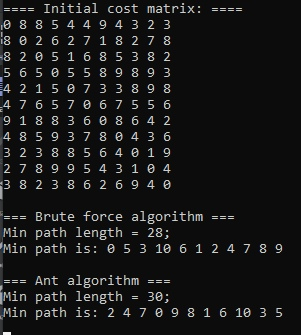
\includegraphics[scale = 0.8]{primer2} \\ Рисунок 4.2: Пример работы программы\\ на матрице размера 11х11
\end{center}	

\section{Параметризация муравьиного алгоритма}

	Для исследования случайным образом была сгенерирована симметричная матрица расстояний размером 12x12. В каждом эксперименте фиксировались значения $\alpha$, $\beta$, $\rho$ и $tmax$. В течение экспериментов коэффициенты $\alpha, \beta, \rho$ менялись от 0 до 1 включительно с шагом 0.25, tmax от 10 до 310 с шагом 20.

\hfill	

Результатом эксперимента считается разница ($diff$) между длинной маршрута, рассчитанного при помощи алгоритма полного перебора и муравьиного алгоритма с определенным набором параметров. Каждый эксперимент проводился 2 раза и в результат записывалось значение длины лучшего найденного пути.

\hfill

В таблице 4.1 представлены результаты эксперимента для параметров $\alpha, \rho$ и $tmax$, строки таблицы отсортированы по возрастанию столбца $diff$. Для наглядности первые 14 строк, давшие лучшие результаты, выделены голубым цветом.
\newpage

\begin{center}
	Таблица 4.1 -- Результаты параметризации муравьиного алгоритма
\end{center}

\begin{center}
	\begin{table}[h!]
		\begin{center}
			\begin{tabular}{|llll|}
				\hline
				\multicolumn{1}{|l|}{$\rho$}                              & \multicolumn{1}{l|}{$\alpha$} & \multicolumn{1}{l|}{$tmax$} & $diff$     \\ \hline
				0.000000 & 0.250000                   & 90.000000                 & 0.000000 \\

				0.000000                                              & 0.500000                   & 250.000000                & 0.000000 \\

				0.000000                                              & 0.750000                   & 290.000000                & 0.000000 \\

				0.000000                                              & 1.000000                   & 330.000000                & 0.000000 \\

				0.250000                                              & 0.000000                   & 210.000000                & 0.000000 \\

				0.250000                                              & 0.250000                   & 210.000000                & 0.000000 \\

				0.250000                                              & 0.500000                   & 170.000000                & 0.000000 \\

				0.250000                                              & 0.500000                   & 330.000000                & 0.000000 \\

				0.250000                                              & 0.750000                   & 330.000000                & 0.000000 \\

				0.500000                                              & 0.000000                   & 250.000000                & 0.000000 \\
 
				0.500000                                              & 0.500000                   & 330.000000                & 0.000000 \\

				0.500000                                              & 0.750000                   & 170.000000                & 0.000000 \\

				0.750000                                              & 0.750000                   & 50.000000                 & 0.000000 \\

				1.000000                                              & 0.250000                   & 50.000000                 & 0.000000 \\ \hline
				0.000000                                              & 0.750000                   & 210.000000                & 2.000000 \\
				1.000000                                              & 0.000000                   & 210.000000                & 2.000000 \\
				1.000000                                              & 0.000000                   & 290.000000                & 2.000000 \\
				0.000000                                              & 0.750000                   & 250.000000                & 2.000000 \\
				1.000000                                              & 0.250000                   & 90.000000                 & 2.000000 \\
				1.000000                                              & 0.250000                   & 130.000000                & 2.000000 \\
				1.000000                                              & 0.500000                   & 130.000000                & 2.000000 \\
				1.000000                                              & 0.500000                   & 250.000000                & 2.000000 \\
				1.000000                                              & 0.500000                   & 290.000000                & 2.000000 \\
				0.000000                                              & 0.000000                   & 250.000000                & 2.000000 \\
				0.000000                                              & 0.750000                   & 330.000000                & 2.000000 \\
				0.000000                                              & 1.000000                   & 50.000000                 & 2.000000 \\
				0.000000                                              & 1.000000                   & 210.000000                & 2.000000 \\
				0.000000                                              & 1.000000                   & 250.000000                & 2.000000 \\
				0.000000                                              & 1.000000                   & 290.000000                & 2.000000 \\
				0.000000                                              & 0.000000                   & 290.000000                & 2.000000 \\
				0.250000                                              & 0.000000                   & 170.000000                & 2.000000 \\
				0.250000                      & 0.000000                   & 290.000000                & 2.000000 \\
				0.000000                      & 0.250000                   & 210.000000                & 2.000000 \\
				0.250000                      & 0.250000                   & 290.000000                & 2.000000 \\
				0.250000                      & 0.250000                   & 330.000000                & 2.000000 \\
				0.000000                      & 0.250000                   & 250.000000                & 2.000000 \\
				0.250000                      & 0.500000                   & 210.000000                & 2.000000 \\
				0.250000                      & 0.500000                   & 250.000000                & 2.000000 \\
				0.000000                                              & 0.000000                   & 170.000000                & 2.000000 \\ \hline
			\end{tabular}
		\end{center}
	\end{table}
	
\end{center}

\newpage


\begin{center}
	
	\begin{table}[h!]
		\begin{center}
			\begin{tabular}{|llll|}
				\hline
				\multicolumn{1}{|l|}{$\rho$}      & \multicolumn{1}{l|}{$\alpha$} & \multicolumn{1}{l|}{$tmax$} & $diff$    \\ \hline
				\multicolumn{1}{|c}{0.250000} & 0.000000                   & 250.000000                & 2.000000 \\
				
				0.250000                      & 0.500000                   & 290.000000                & 2.000000 \\
				0.000000                      & 0.250000                   & 290.000000                & 2.000000 \\
				0.250000                      & 0.750000                   & 90.000000                 & 2.000000 \\
				0.250000                      & 0.750000                   & 130.000000                & 2.000000 \\
				0.250000                      & 0.750000                   & 170.000000                & 2.000000 \\
				0.250000                      & 0.750000                   & 210.000000                & 2.000000 \\
				0.250000                      & 0.750000                   & 250.000000                & 2.000000 \\
				0.250000                      & 0.750000                   & 290.000000                & 2.000000 \\
				0.000000                      & 0.250000                   & 330.000000                & 2.000000 \\
				0.250000                      & 1.000000                   & 90.000000                 & 2.000000 \\
				0.250000                      & 1.000000                   & 210.000000                & 2.000000 \\
				0.250000                      & 1.000000                   & 250.000000                & 2.000000 \\
				0.250000                      & 1.000000                   & 290.000000                & 2.000000 \\
				0.250000                      & 1.000000                   & 330.000000                & 2.000000 \\
				0.500000                      & 0.000000                   & 90.000000                 & 2.000000 \\
				0.000000                      & 0.500000                   & 170.000000                & 2.000000 \\
				0.500000                      & 0.000000                   & 290.000000                & 2.000000 \\
				0.500000                      & 0.250000                   & 330.000000                & 2.000000 \\
				0.500000                      & 0.500000                   & 250.000000                & 2.000000 \\
				0.500000                      & 0.500000                   & 290.000000                & 2.000000 \\
				0.000000                      & 0.000000                   & 210.000000                & 2.000000 \\
				0.000000                      & 0.500000                   & 290.000000                & 2.000000 \\
				0.500000                      & 1.000000                   & 170.000000                & 2.000000 \\
				0.500000                      & 1.000000                   & 210.000000                & 2.000000 \\
				0.500000                      & 1.000000                   & 290.000000                & 2.000000 \\
				0.750000                      & 0.000000                   & 170.000000                & 2.000000 \\
				0.750000                      & 0.250000                   & 130.000000                & 2.000000 \\
				0.750000                      & 0.250000                   & 250.000000                & 2.000000 \\
				0.750000                      & 0.500000                   & 170.000000                & 2.000000 \\
				0.750000                      & 0.500000                   & 250.000000                & 2.000000 \\
				1.000000                      & 0.250000                   & 290.000000                & 3.000000 \\
				1.000000                      & 0.250000                   & 330.000000                & 3.000000 \\
				0.250000                      & 0.250000                   & 130.000000                & 3.000000 \\
				1.000000                      & 0.500000                   & 210.000000                & 3.000000 \\
				0.250000                      & 0.250000                   & 170.000000                & 3.000000 \\
				0.000000                      & 0.250000                   & 130.000000                & 3.000000 \\
				1.000000                      & 0.750000                   & 330.000000                & 3.000000 \\
				0.250000                      & 0.250000                   & 250.000000                & 3.000000 \\
				0.500000                      & 0.000000                   & 210.000000                & 3.000000 \\
				0.000000                      & 0.500000                   & 130.000000                & 3.000000 \\
				1.000000                      & 0.750000                   & 130.000000                & 3.000000 \\ \hline
			\end{tabular}
		\end{center}
	\end{table}
	
\end{center}

\newpage

\begin{center}
	
	\begin{table}[h!]
		\begin{center}
			\begin{tabular}{|llll|}
				\hline
				\multicolumn{1}{|l|}{$\rho$}      & \multicolumn{1}{l|}{$\alpha$} & \multicolumn{1}{l|}{$tmax$} & $diff$      \\ \hline
				\multicolumn{1}{|c}{1.000000} & 0.750000                   & 290.000000                & 3.000000 \\
				0.000000                      & 0.250000                   & 170.000000                & 3.000000 \\
				0.500000                      & 0.250000                   & 90.000000                 & 3.000000 \\
				0.500000                      & 0.250000                   & 250.000000                & 3.000000 \\
				0.250000                      & 0.500000                   & 50.000000                 & 3.000000 \\
				0.500000                      & 0.500000                   & 50.000000                 & 3.000000 \\
				0.500000                      & 0.500000                   & 90.000000                 & 3.000000 \\
				0.500000                      & 0.500000                   & 130.000000                & 3.000000 \\
				0.250000                      & 0.500000                   & 130.000000                & 3.000000 \\
				0.000000                      & 0.500000                   & 210.000000                & 3.000000 \\
				0.000000                      & 1.000000                   & 90.000000                 & 3.000000 \\
				0.000000                      & 1.000000                   & 170.000000                & 3.000000 \\
				0.500000                      & 0.750000                   & 250.000000                & 3.000000 \\
				0.500000                      & 0.750000                   & 290.000000                & 3.000000 \\
				0.000000                      & 0.000000                   & 90.000000                 & 3.000000 \\
				0.000000                      & 0.000000                   & 330.000000                & 3.000000 \\
				0.500000                      & 1.000000                   & 250.000000                & 3.000000 \\
				0.250000                      & 0.750000                   & 50.000000                 & 3.000000 \\
				0.500000                      & 1.000000                   & 330.000000                & 3.000000 \\
				0.000000                      & 0.500000                   & 330.000000                & 3.000000 \\
				0.750000                      & 0.000000                   & 210.000000                & 3.000000 \\
				0.750000                      & 0.000000                   & 290.000000                & 3.000000 \\
				0.750000                      & 0.000000                   & 330.000000                & 3.000000 \\
				0.000000                      & 0.750000                   & 50.000000                 & 3.000000 \\
				0.750000                      & 0.250000                   & 170.000000                & 3.000000 \\
				0.750000                      & 0.250000                   & 210.000000                & 3.000000 \\
				0.250000                      & 0.000000                   & 90.000000                 & 3.000000 \\
				0.750000                      & 0.250000                   & 290.000000                & 3.000000 \\
				0.750000                      & 0.250000                   & 330.000000                & 3.000000 \\
				0.750000                      & 0.500000                   & 130.000000                & 3.000000 \\
				0.000000                      & 0.750000                   & 90.000000                 & 3.000000 \\
				0.000000                      & 0.750000                   & 130.000000                & 3.000000 \\
				0.750000                      & 0.500000                   & 290.000000                & 3.000000 \\
				0.750000                      & 0.500000                   & 330.000000                & 3.000000 \\
				0.000000                      & 0.750000                   & 170.000000                & 3.000000 \\
				0.750000                      & 0.750000                   & 330.000000                & 3.000000 \\
				1.000000                      & 0.000000                   & 90.000000                 & 3.000000 \\
				0.000000                      & 0.000000                   & 50.000000                 & 3.000000 \\
				1.000000                      & 0.000000                   & 250.000000                & 3.000000 \\
				0.250000                      & 0.000000                   & 330.000000                & 3.000000 \\
				1.000000                      & 0.000000                   & 330.000000                & 3.000000 \\
				0.250000                      & 1.000000                   & 130.000000                & 3.000000 \\ \hline
			\end{tabular}
		\end{center}
	\end{table}
	
\end{center}

\newpage

\begin{table}[h!]
	\begin{center}
		\begin{tabular}{|llll|}
			\hline
			\multicolumn{1}{|l|}{$\rho$}      & \multicolumn{1}{l|}{$\alpha$} & \multicolumn{1}{l|}{$tmax$} & $diff$     \\ \hline
			\multicolumn{1}{|c}{0.250000} & 1.000000                   & 170.000000                & 3.000000 \\
			0.250000                      & 0.250000                   & 90.000000                 & 3.000000 \\
			1.000000                      & 0.250000                   & 210.000000                & 3.000000 \\
			0.000000                      & 0.500000                   & 90.000000                 & 4.000000 \\
			0.500000                      & 0.250000                   & 130.000000                & 4.000000 \\
			0.500000                      & 0.250000                   & 170.000000                & 4.000000 \\
			1.000000                      & 0.250000                   & 170.000000                & 4.000000 \\
			0.500000                      & 0.250000                   & 210.000000                & 4.000000 \\
			1.000000                      & 0.250000                   & 250.000000                & 4.000000 \\
			0.750000                      & 0.000000                   & 10.000000                 & 4.000000 \\
			0.750000                      & 0.000000                   & 130.000000                & 4.000000 \\
			0.250000                      & 0.750000                   & 10.000000                 & 4.000000 \\
			0.500000                      & 0.250000                   & 290.000000                & 4.000000 \\
			0.750000                      & 0.000000                   & 250.000000                & 4.000000 \\
			0.000000                      & 0.000000                   & 10.000000                 & 4.000000 \\
			0.250000                      & 0.250000                   & 50.000000                 & 4.000000 \\
			1.000000                      & 0.750000                   & 170.000000                & 4.000000 \\
			1.000000                      & 0.750000                   & 250.000000                & 4.000000 \\
			0.750000                      & 0.250000                   & 50.000000                 & 4.000000 \\
			0.250000                      & 0.500000                   & 90.000000                 & 4.000000 \\
			0.000000                      & 1.000000                   & 130.000000                & 4.000000 \\
			0.500000                      & 0.500000                   & 170.000000                & 4.000000 \\
			0.500000                      & 0.500000                   & 210.000000                & 4.000000 \\
			0.250000                      & 0.000000                   & 130.000000                & 4.000000 \\
			0.000000                      & 0.250000                   & 50.000000                 & 4.000000 \\
			0.750000                      & 0.500000                   & 50.000000                 & 4.000000 \\
			0.500000                      & 0.000000                   & 130.000000                & 4.000000 \\
			0.500000                      & 0.750000                   & 50.000000                 & 4.000000 \\
			0.750000                      & 0.500000                   & 210.000000                & 4.000000 \\
			0.500000                      & 0.750000                   & 130.000000                & 4.000000 \\
			0.000000                      & 0.000000                   & 130.000000                & 4.000000 \\
			0.500000                      & 0.750000                   & 210.000000                & 4.000000 \\
			0.000000                      & 0.500000                   & 50.000000                 & 4.000000 \\
			0.750000                      & 0.750000                   & 130.000000                & 4.000000 \\
			0.750000                      & 0.750000                   & 210.000000                & 4.000000 \\
			0.250000                      & 1.000000                   & 50.000000                 & 4.000000 \\
			0.750000                      & 1.000000                   & 50.000000                 & 4.000000 \\
			0.750000                      & 1.000000                   & 250.000000                & 4.000000 \\
			0.750000                      & 1.000000                   & 330.000000                & 4.000000 \\
			1.000000                      & 0.000000                   & 50.000000                 & 4.000000 \\
			0.500000                      & 0.750000                   & 330.000000                & 4.000000 \\
			1.000000                      & 0.000000                   & 130.000000                & 4.000000 \\
			1.000000                      & 0.000000                   & 170.000000                & 4.000000 \\
			0.500000                      & 1.000000                   & 50.000000                 & 4.000000 \\
			0.500000                      & 1.000000                   & 90.000000                 & 4.000000 \\ \hline
		\end{tabular}
	\end{center}
\end{table}

\newpage

\begin{center}
	
	\begin{table}[h!]
		\begin{center}
			\begin{tabular}{|llll|}
				\hline
				\multicolumn{1}{|l|}{$\rho$}      & \multicolumn{1}{l|}{$\alpha$} & \multicolumn{1}{l|}{$tmax$} & $diff$      \\ \hline
				\multicolumn{1}{|c}{0.500000} & 1.000000                   & 130.000000                & 4.000000 \\
				0.500000                      & 0.000000                   & 330.000000                & 4.000000 \\
				0.750000                      & 0.000000                   & 90.000000                 & 5.000000 \\
				1.000000                      & 0.500000                   & 170.000000                & 5.000000 \\
				0.750000                      & 0.250000                   & 10.000000                 & 5.000000 \\
				0.750000                      & 0.500000                   & 10.000000                 & 5.000000 \\
				0.750000                      & 0.750000                   & 90.000000                 & 5.000000 \\
				1.000000                      & 0.500000                   & 330.000000                & 5.000000 \\
				0.500000                      & 0.750000                   & 90.000000                 & 5.000000 \\
				0.750000                      & 0.750000                   & 170.000000                & 5.000000 \\
				1.000000                      & 0.750000                   & 210.000000                & 5.000000 \\
				0.750000                      & 0.500000                   & 90.000000                 & 5.000000 \\
				0.750000                      & 0.750000                   & 250.000000                & 5.000000 \\
				0.750000                      & 0.750000                   & 290.000000                & 5.000000 \\
				1.000000                      & 1.000000                   & 50.000000                 & 5.000000 \\
				1.000000                      & 1.000000                   & 210.000000                & 5.000000 \\
				1.000000                      & 1.000000                   & 250.000000                & 5.000000 \\
				1.000000                      & 1.000000                   & 290.000000                & 5.000000 \\
				1.000000                      & 1.000000                   & 330.000000                & 5.000000 \\
				0.500000                      & 0.000000                   & 170.000000                & 5.000000 \\
				0.250000                      & 0.000000                   & 50.000000                 & 5.000000 \\
				0.750000                      & 1.000000                   & 130.000000                & 5.000000 \\
				0.750000                      & 1.000000                   & 210.000000                & 5.000000 \\
				0.500000                      & 0.000000                   & 50.000000                 & 5.000000 \\
				0.750000                      & 1.000000                   & 290.000000                & 5.000000 \\
				0.750000                      & 0.000000                   & 50.000000                 & 5.000000 \\
				0.750000                      & 1.000000                   & 170.000000                & 6.000000 \\
				1.000000                      & 0.000000                   & 10.000000                 & 6.000000 \\
				0.250000                      & 0.500000                   & 10.000000                 & 6.000000 \\
				1.000000                      & 0.500000                   & 50.000000                 & 6.000000 \\
				1.000000                      & 0.750000                   & 50.000000                 & 6.000000 \\
				1.000000                      & 0.750000                   & 90.000000                 & 6.000000 \\
				1.000000                      & 0.500000                   & 90.000000                 & 6.000000 \\
				0.750000                      & 1.000000                   & 90.000000                 & 6.000000 \\
				0.500000                      & 0.500000                   & 10.000000                 & 6.000000 \\
				0.000000                      & 0.250000                   & 10.000000                 & 7.000000 \\
				0.250000                      & 1.000000                   & 10.000000                 & 7.000000 \\
				0.750000                      & 0.250000                   & 90.000000                 & 7.000000 \\
				1.000000                      & 1.000000                   & 130.000000                & 7.000000 \\
				1.000000                      & 1.000000                   & 170.000000                & 7.000000 \\
				0.500000                      & 0.250000                   & 50.000000                 & 7.000000 \\
				0.500000                      & 0.000000                   & 10.000000                 & 7.000000 \\
				0.000000                      & 0.500000                   & 10.000000                 & 8.000000 \\
				1.000000                      & 0.500000                   & 10.000000                 & 8.000000 \\
				1.000000                      & 1.000000                   & 10.000000                 & 8.000000 \\ \hline
			\end{tabular}
		\end{center}
	\end{table}
	
	
\end{center}

\newpage

\begin{center}
	
	\begin{table}[h!]
		\begin{center}
			\begin{tabular}{|llll|}
				\hline
				\multicolumn{1}{|l|}{$\rho$}      & \multicolumn{1}{l|}{$\alpha$} & \multicolumn{1}{l|}{$tmax$} & $diff$      \\ \hline
				\multicolumn{1}{|c}{1.000000} & 0.250000                   & 10.000000                 & 8.000000  \\
				1.000000                      & 1.000000                   & 90.000000                 & 8.000000  \\
				0.250000                      & 0.250000                   & 10.000000                 & 8.000000  \\
				0.000000                      & 0.750000                   & 10.000000                 & 9.000000  \\
				0.250000                      & 0.000000                   & 10.000000                 & 9.000000  \\
				0.750000                      & 1.000000                   & 10.000000                 & 10.000000 \\
				0.500000                      & 1.000000                   & 10.000000                 & 10.000000 \\
				0.500000                      & 0.250000                   & 10.000000                 & 10.000000 \\
				0.500000                      & 0.750000                   & 10.000000                 & 11.000000 \\
				0.750000                      & 0.750000                   & 10.000000                 & 11.000000 \\
				1.000000                      & 0.750000                   & 10.000000                 & 11.000000 \\
				0.000000                      & 1.000000                   & 10.000000                 & 12.000000 \\ \hline
			\end{tabular}
		\end{center}
	\end{table}
	
\end{center}

\clearpage
\newpage

	Из результатов таблицы 4.1 можно выделить оптимальные коэффициенты $\alpha$, $\rho$, значение $tmax$; результат анализа отражен в таблице 4.2.

\begin{center}
	Таблица 4.2 -- Оптимальные коэффициенты муравьиного алгоритма
\end{center}

\begin{center}
	\begin{table}[h!]
		\begin{center}
			\begin{tabular}{|l|l|l|}
				\hline
				$\rho$                        & $\alpha$ & $tmax$ \\ \hline
				\multicolumn{1}{|c|}{0.25} & 0.5   & 170  \\ \hline
				0.25                       & 0.5   & 330  \\ \hline
				0.5                        & 0.5   & 330  \\ \hline
				0.5                        & 0.75  & 170  \\ \hline
			\end{tabular}
		\end{center}
	\end{table}
	
\end{center}

\section{Сравнение времени работы}

\hfill

На графиках (рисунки 4.3 и 4.4) представлено сравнение времени работы алгоритма полного перебора и муравьиного алгоритма с вычисленными параметрами $\rho = 0.25$, $\alpha = 0.5$, $tmax = 170$. 

На первом графике (рисунок 4.3) исследование происходило на матрицах размера 2х2, 3х3, 4х4, ..., 11х11.

На втором графике (рисунок 4.4) исследование происходило на матрицах размера 2х2, 3х3, 4х4, ..., 8х8.

\begin{center}
	\label{img:graph} 
	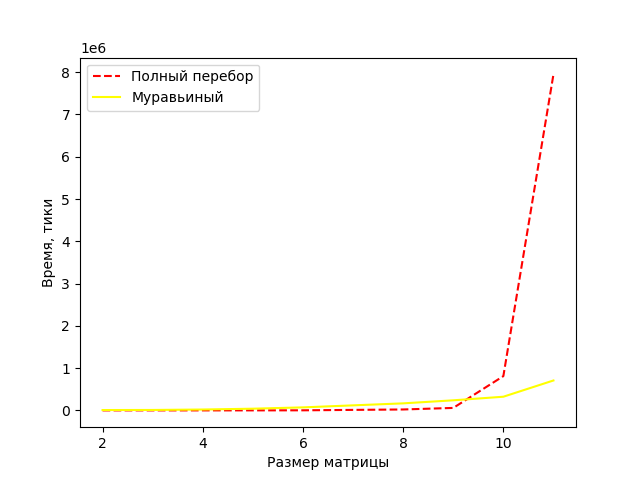
\includegraphics[scale = 0.9]{graph} \\ Рисунок 4.3 -- Сравнение времени работы алгоритма полного перебора \\и муравьиного алгоритма на матрицах 2х2, ..., 11х11.
\end{center}

\begin{center}
	\label{img:graph2} 
	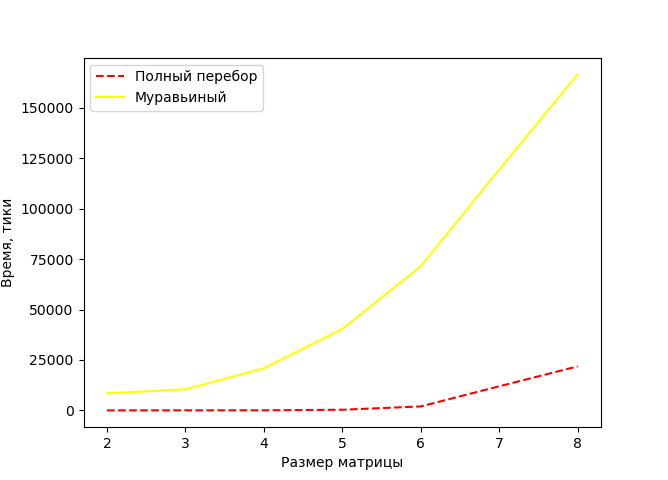
\includegraphics[scale = 0.94]{graph2} \\ Рисунок 4.4 -- Сравнение времени работы алгоритма полного перебора \\и муравьиного алгоритма на матрицах 2х2, ..., 8х8.
\end{center}


\section{Вывод}

В результате проведенных экспериментов были найдены оптимальные параметры для муравьиного алгоритма.
Муравьиный алгоритм дает лучшие результаты при 

$0.25 \leq  \rho \leq 0.5$,

$0.5 \leq  \alpha \leq 0.75$,

$170 \leq  tmax \leq 330$. 

\hfill

При этом чем больше значение $tmax$, тем больше вероятность того, что будет найден самый короткий маршрут. 

\hfill

Также проведен сравнительный анализ времения работы муравьиного алгоритма и алгоритма полного перебора.
По скорости муравьиный алгоритм сильно выигрывает у алгоритма полного перебора, на матрицах, размер которых превышает 10х10.

\hfill

Алгоритм полного перебора стоит использовать, если:
\begin{enumerate}
	\item[1)] матрицы имеют размер, меньший чем 10х10 элементов;
	\item[2)] в задачах, где нужно гарантированно найти самый короткий путь.
\end{enumerate}  


\chapter*{Заключение}
\addcontentsline{toc}{chapter}{Заключение}

Задача коммивояжера -- одна из важных задач комбинаторики и пользуется популярностью благодаря тому, что к ней сводится большое количество практических задач. Она была выбрана первой для решения с использованием подхода, заимствующего механизмы поведения муравьиной колонии. Позже этот подход нашел применение в решении других комбинаторных проблем, в числе которых задачи о назначениях, задача раскраски графа, задачи маршрутизации, задачи из областей data mining и распознавания образов и другие.

Проведенные опыты показали, что критерий выбора алгоритма для расчета маршрута будет зависеть от количества городов N:
\begin{enumerate}
	\item при $N < 10$ поиск маршрута целесообразно осуществлять с помощью алгоритма полного перебора, так как он дает точное решение задачи коммивояжера, не проигрывая при этом по времени муравьиному алгоритму;
	\item при $N > 10$ поиск маршрута целесообразно осуществлять с помощью муравьиного алгоритма, так как он работает быстрее алгоритма полного перебора, но при этом муравьиный алгоритм зависит от настроечных параметров, которые подбираются только исходя из экспериментов.
\end{enumerate}

При выполнении лабораторной работы цель была достигнута: проведен сравнительный анализ метода полного перебора и эвристического метода на базе муравьиного алгоритма.

Также были выполнены следующие задачи: 
\begin{enumerate} 
	\item реализованы методыы полного перебора и метод на базе муравьиного алгоритма для решения задачи коммивояжёра;
	\item проведена параметризация метода на базе муравьиного алгоритма для выбранного класса задач, т.е. определены комбинации параметров, при которых метод даёт наилучшие результаты на выбранном классе задач;
	\item произведено сравнение алгоритма полного перебора и муравьиного по скорости работы.
\end{enumerate} .

\addcontentsline{toc}{chapter}{Список литератури}

\bibliographystyle{utf8gost705u}  % стилевой файл для оформления по ГОСТу

\bibliography{51-biblio}          % имя библиографической базы (bib-файла)

\begin{thebibliography}{9}
	\addcontentsline{toc}{section}{Литература}
	\bibitem{link1} Новиков Ф.А. Дискретная математика для программистов . –  СПб.: Изд-во Питер, 2012. – 208 с.
	\bibitem{link3} Майника Э. Алгоритмы оптимизации на сетях и графах. – СПб.: М.: Мир,
	1981. – 323 с.
	\bibitem{link4} Vector в C++: основные приемы эффективного использования [Электронный ресурс]. - Режим доступа: https://codelessons.ru/cplusplus/vektory-v-c-dlya-nachinayushhix.html (дата обращения: 03.12.2020)
	\bibitem{link6} Полиномиальные алгоритмы и задачи [Электронный ресурс]. - Режим доступа: https://studfile.net/preview/5562531/page:41/ (дата обращения: 22.12.2020)
	
\end{thebibliography}

\end{document}
